\subsection{Fault tolerance techinques}\label{subsec:archtolerance}

For each module of the Erlang subsystem some techniques have been implemented to
ensure a good degree of availability and tolerance to tastes.

\figref{fig:erlang-arch2} shows the Erlang subsystem's architecture.

\begin{figure}[htb]
	\centering
	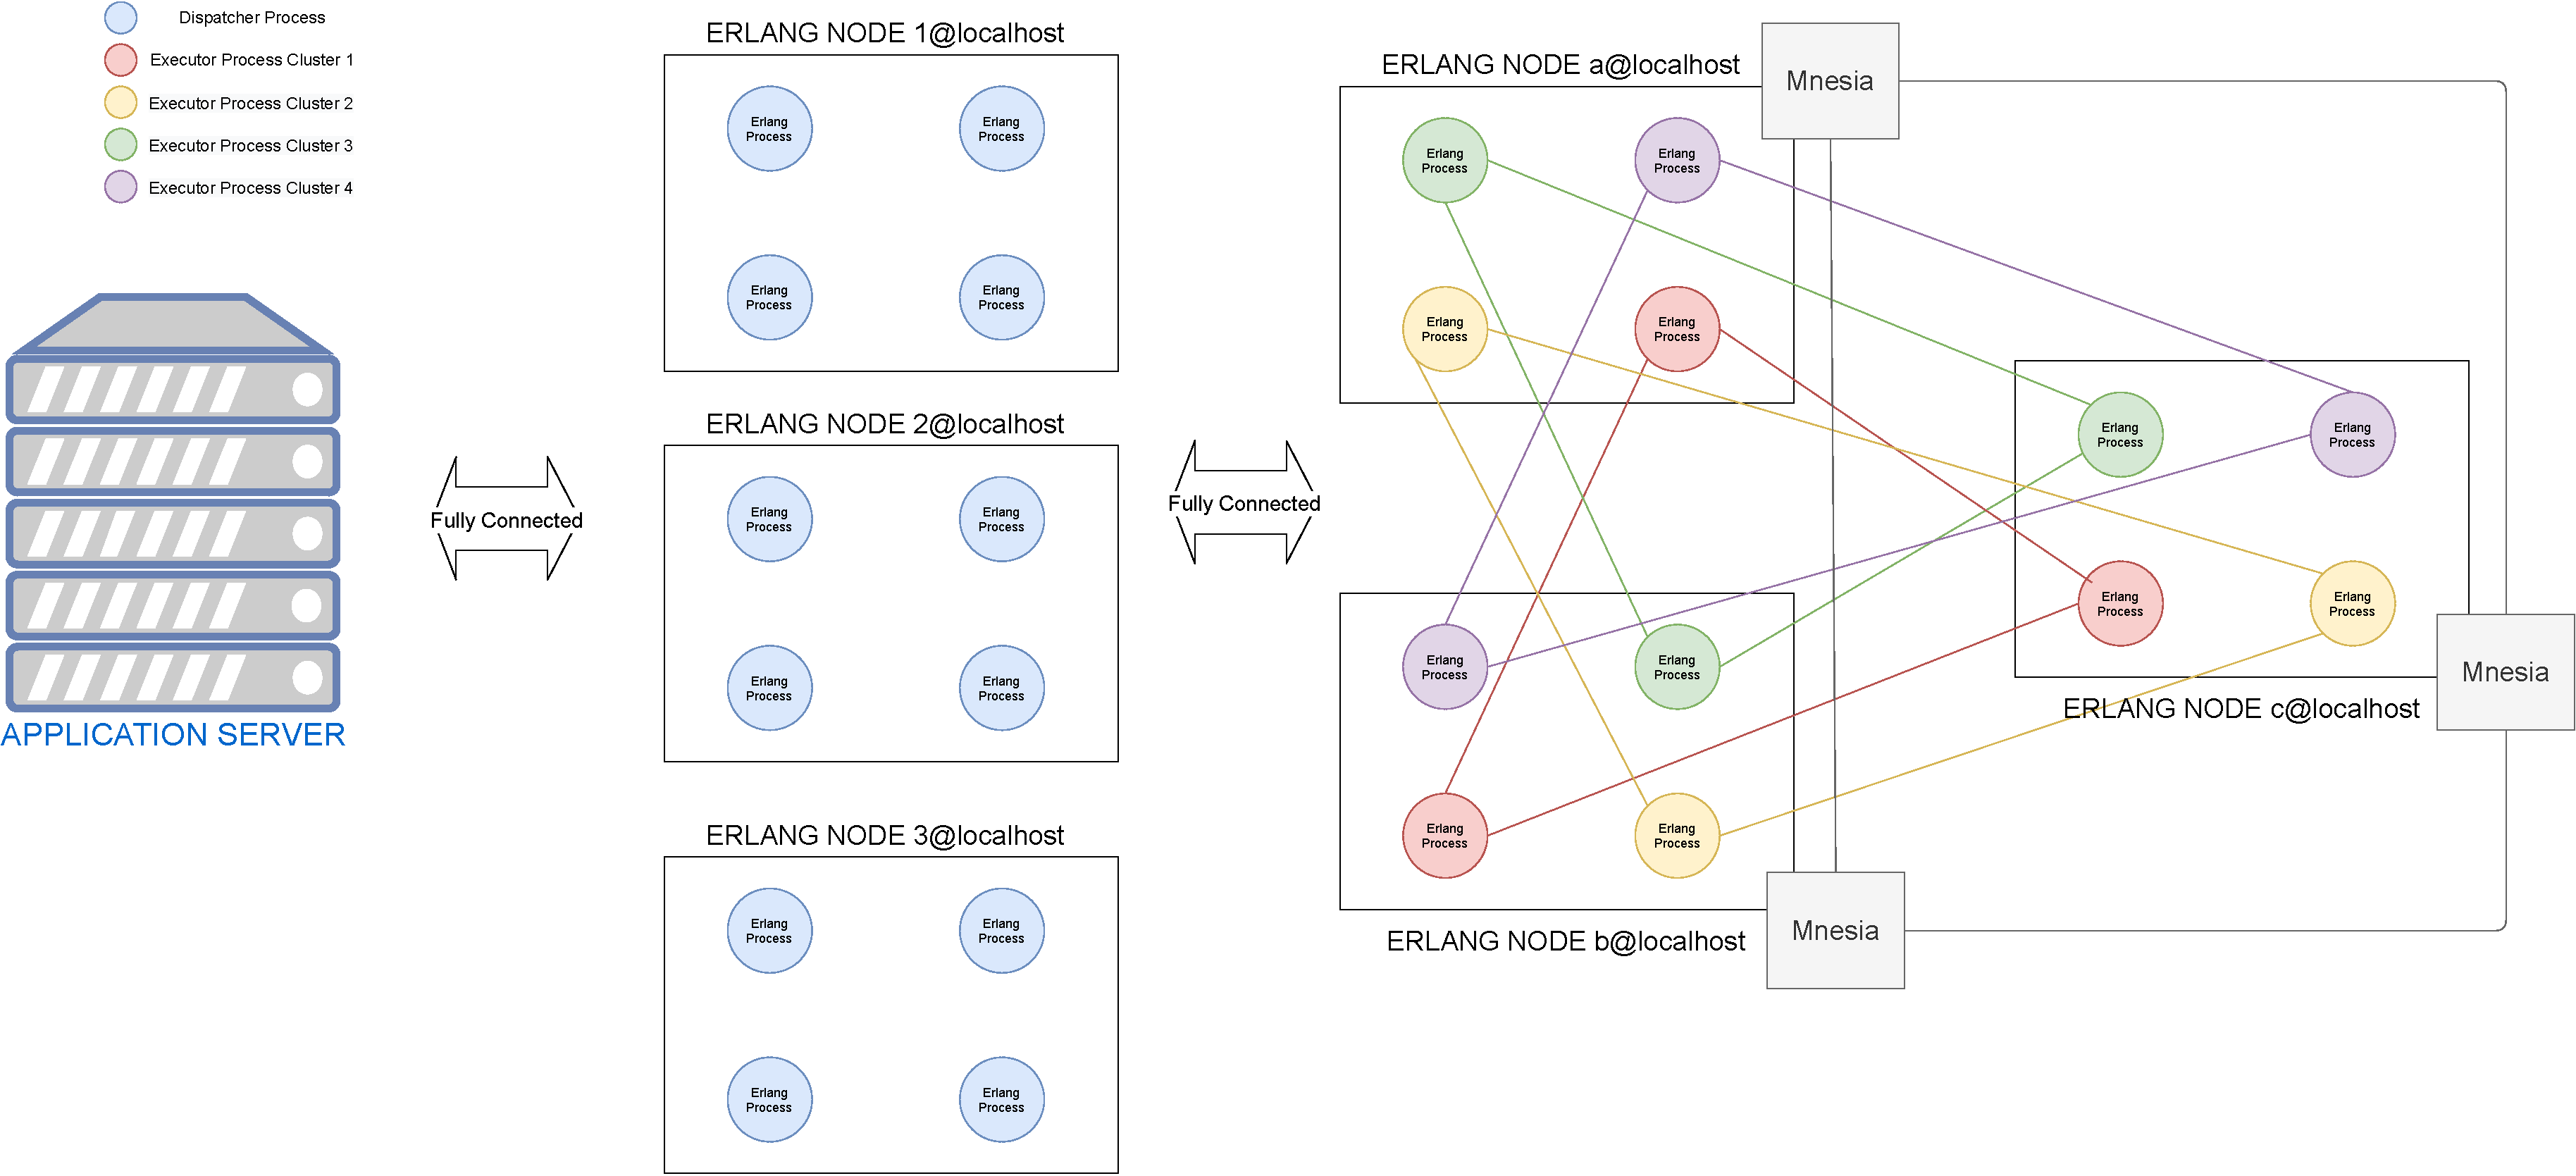
\includegraphics[width=\textwidth]{erlang-arch2}
	\caption{Erlang subystem architecture}\label{fig:erlang-arch2}
\end{figure}

\subsubsection{Dispatchers}

As can be seen from the architecture, multiple dispatcher instances are executed
on different dispatcher Erlang nodes to allow the application server to always
find an available dispatcher in case a dispatcher process/node fails.
Furthermore, the presence of multiple dispatcher instances allows the
application server to implement load-balancing techniques to balance the load of
requests between the dispatchers available;

\subsubsection{Executor clusters}

Each executor cluster is organized according to a \textbf{leader-slaves
structure}. The leader manages the requests coming from the dispatchers,
communicate (if needed) to the Mnesia for the persistence of data, and calculate
the current \code{AuctionState} of the auctions and then sends it to the slaves.
The slaves have the function of replicas.

If the leader fails, the slaves will start a leader election process using the
\textbf{Bully algorithm}, to allow the cluster to remain operational.

\figref{fig:bully-state} shows the Bully algorithm state machine implemented in
this application.

\begin{figure}[htb]
	\centering
	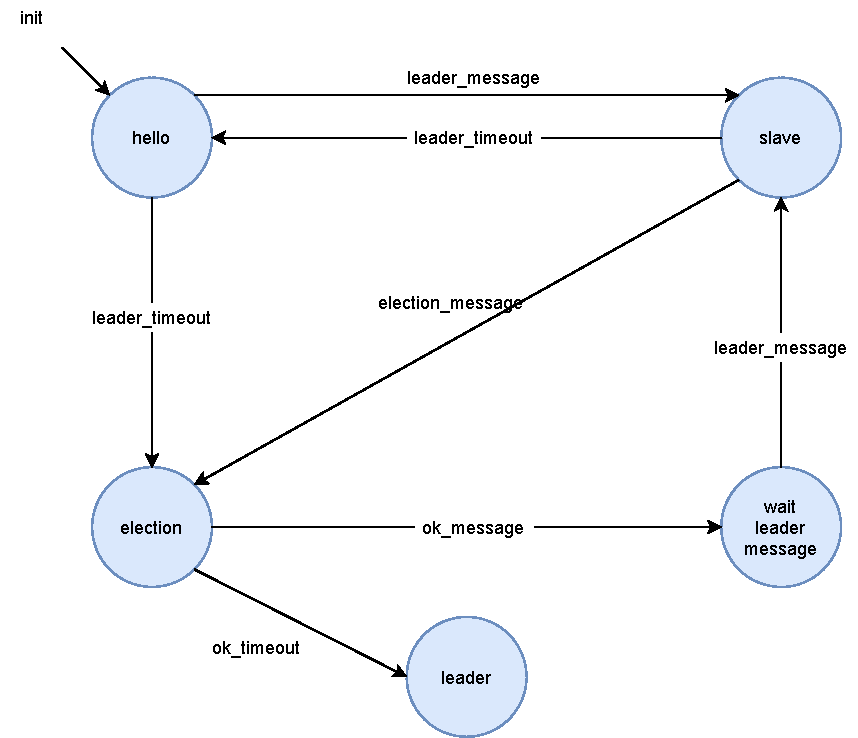
\includegraphics[width=\textwidth]{bully-state}
	\caption{Bully Algorithm State Machine}\label{fig:bully-state}
\end{figure}

Furthermore, as is visible from the architecture, the processes of each executor
cluster are executed in different executor Erlang nodes (even if it is possible
that the same node executes more processes of the same cluster) so that the
clusters continue their operation even in case of failure of an executor Erlang
node.
